\textbf{Parte II - Los estudiantes contestarán las siguientes preguntas propuestas.
}

Pág. 53 del libro

\begin{enumerate}
    \item \textbf{¿Qué se entiende por grados de libertad de un robot? Dibuje el esquema de un robot manipulador con 4 DOF.}

    R: Cada uno de los movimientos independientes que puede realizar cada articulación con respecto a la anterior.

    \begin{figure}[H]
        \centering
        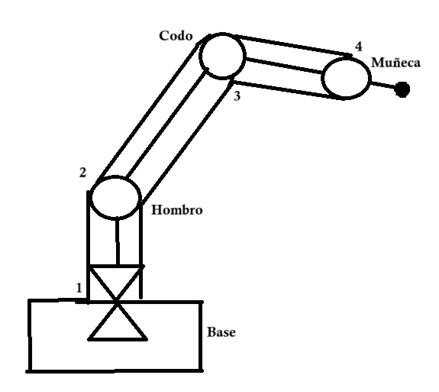
\includegraphics[scale = 0.90]{Imagenes/p1.png}
        \caption{Esquema de un robot manipulador con 4 DOF}{Fuente: Internet}
    \end{figure}

    \item \textbf{Defina con sus propias palabras las siguientes características de un robot industrial: resolución, precisión, repetibilidad, volumen de trabajo y capacidad de carga.}
    
    \begin{itemize}


        \item Precisión: Es la diferencia entre la posición alcanzada y la posición ordenada del robot. 
        \item Resolución: Es la menor variación en el posicionamiento del extremo del robot, es la precisión mínima con la que el robot puede moverse. 
        \item Repetibilidad: Se refiere a la capacidad del robot de volver a la misma posición la cantidad de veces que sea. Esta característica es muy importante porque no importa si el robot alcanzo su objetivo una vez, la idea es que lo logre las veces que sea.
        \item Volumen de trabajo: Es el alcance que tiene programado el robot para moverse y hacer sus tareas.
        \item Capacidad de carga: Es el peso máximo que un robot puede desplazar, eso incluyendo a la misma herramienta que tenga el robot. 
        
    \end{itemize}

    \item \textbf{Explique la diferencia entre los conceptos de precisión (exactitud)  y repetibilidad de un robot industrial. Emplee un dibujo para aclararlo. }
    
    R: Si un robot tiene precisión, cada vez que se le asigne una tarea, intentara hacerla lo mas completa posible y si es repetitivo entonces lograr a llegar a esa misma posición (en este caso el objetivo de la tarea u otra cosa) las veces que se le haya pedido.

    \begin{figure}[H]
        \centering
        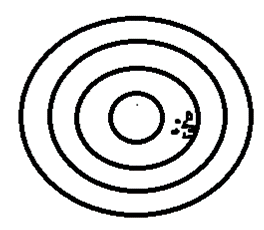
\includegraphics[scale = 0.5]{Imagenes/repeti.png}
        \caption{Repetibildiad}{Fuente:Internet}
    \end{figure}

    \begin{figure}[H]
        \centering
        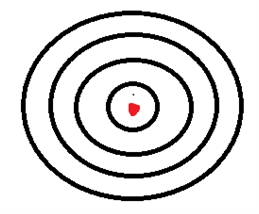
\includegraphics[scale = 0.5]{Imagenes/presicion.png}
        \caption{Precisión}{Fuente:Internet}
    \end{figure}

    \item \textbf{Enumere y describa los distintos tipos posible de articulaciones de un robot industrial.}
    
    \begin{itemize}
        \item Rótula: Permite movimiento de rotación alrededor de múltiples ejes, similar a una bola en un soporte.
        \item Prismática: permite el movimiento de traslación lineal a lo largo de un eje. 
        \item Cilíndrica: Combina una rotación alrededor de un eje y un movimiento lineal a lo largo de ese mismo eje. 
        \item Planar: Permite un movimiento de traslación en dos dimensiones, a lo largo de un plano (X, Y).
        \item Tornillo: combinación de movimientos de rotación y traslación lineal.
        \item Rotación: permite únicamente el movimiento rotacional alrededor de un eje fijo.
    \end{itemize}

    \item \textbf{Explique qué tipo de robot responde a las siguientes características: posee control de posición por topes mecánicos, su accionamiento es habitualmente neumático realizando movimientos cíclicos repetitivos de pick y place. Indique la diferencia entre un AGV y un robot móvil autónomo.}
    
    \begin{enumerate}
        \item robot secuencial. 
        \item los AGV son para carga en células robóticas y tienen una ruta predefinida y los robots móviles autónomos se desplazan de manera autónoma en su entorno.

    \end{enumerate}

    


\end{enumerate}

